\section{Beyond Our Blacklists}
\label{sec:large-scale}

%In this section we analyze how fast does different network update their blocking policy.
%So far the goal of our measurement was to infer if a {\reflector} uses a
%specific blacklist to block traffic. While this informs our view of the usage
%of specific blacklists it does not inform our broader perspective on the
%usage of threat intelligence at large. Essentially, in this section we would
%like to see if any of our {\reflectors} use any blacklist, or implement any
%security features that involves IP-based traffic blocking.

%During our measurement, we looked at over 100 public IP blacklists, but there
%is a wide selection of commercial blacklists that we cannot cover. In order
%to look at the blocking behavior from a wider lens, we would like to test
%blacklist IPs that are shared by as many products as possible. Of course,
%there is no concrete way to identify these IPs, so we try to use some
%heuristic to increase the likelihood that the IPs selected are also covered
%by other blacklists.

%In order to accomplish this, we still sample IPs from the top 9 blacklist we
%identified, but instead of selecting exclusive IPs, we sample from the
%\textit{nonexclusive} portion of each blacklists, so that these IPs are
%shared with at least one more blacklist. We further reduce the candidate pool
%by only keeping the IPs that have stayed in the blacklist for at least 3
%weeks. Being ``shared'' and ``stable'' are the heuristics we use to increase
%the chances that these IPs are also shared with many other blacklists. We
%then drop the IPs that are not routable or are from the {\reflector} AS.
%Finally, we randomly sample 80 IPs from the remaining IPs for our experiment.
%We test these IPs against all our {\reflectors} to identify blocking
%behaviors. To be conservative, we conduct this experiment twice and use two
%different set of randomly selected 80 IPs. Additionally, each time we also
%include a control group, where we randomly select 80 IPs from
%\textcolor{red}{Explain how control group come.}

\begin{figure}[t]
\centering
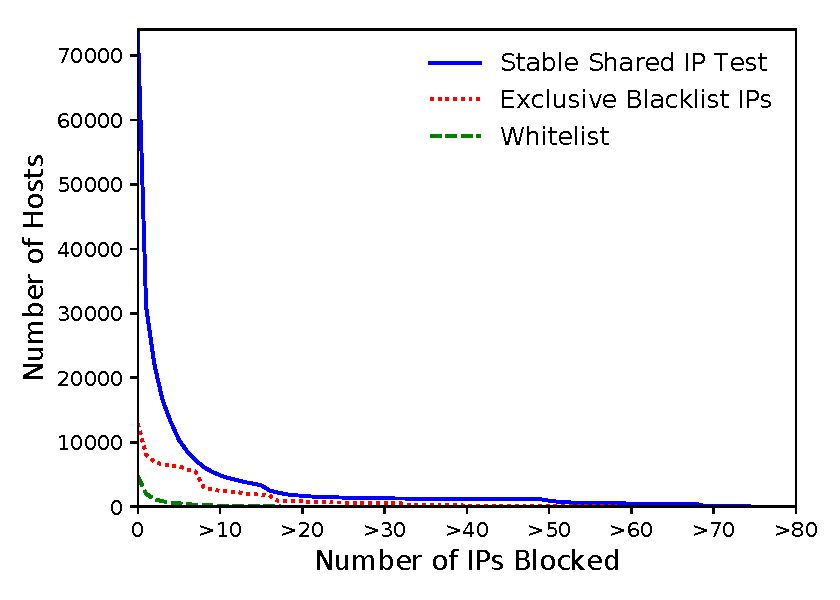
\includegraphics[width=0.8\columnwidth]{data_usage/images/large_scale_rcdf_v2.pdf}
\caption{Number of {\reflectors} ($y$-axis) that block at least
  some number of blacklist IPs ($x$-axis)}
\label{fig:large_scale_rcdf}
\end{figure}


Previously we chose blacklist IPs that were exclusive to each
blacklist, effectively creating a set of IPs that served as a
signature for that blacklist. But as we can see from Figure~\ref{fig:reflector-breakdown},
there are over 20\% of {\reflectors} that blocked at least one
blacklist IP during one of the three experiments, and we do not
have a clear explanation. One possible case is that the blacklist IPs
we sampled happen to overlap with some commercial blacklists we
do not know, and those lists are more widely used. To check this
possibility, we change our blacklist IP sampling criteria and conduct
a new experiment.

Now our goal is the opposite: we want
to choose among common, or shared, IPs that appear on multiple
blacklists.  As added caution, we also focus on shared IPs that are
the most stable, appearing on the blacklists for at least three weeks.
Our goal is to bias selecting blacklist IPs that are so egregiously
suspicious that not only do they appear on multiple of our public
blacklists for a long period of time, but as a result they also likely
appear on other public and commercial blacklists that we do not have
access to.

% \noteby{GV}{Opportunity for an analogy here.}

For this experiment we randomly selected 80 blacklist IPs that appear
on more than one blacklist and, as with previous experiments, that are
routable and AS disjoint.  We refer to this set as the ``Shared''
blacklist IPs.  For comparison, we also randomly selected a set of 80
blacklist IPs from our previous experiment, the ones that are
exclusive to one blacklist (``Exclusive''), and a random set of 80 IPs
as a whitelist set (``Whitelist''), again with the routable and AS disjoint
criteria. Here the whitelist is constructed by randomly sampling IPs
from top 10,000 most visited IPs among all the network traffic in our own
organization in one day (an education institute of over 30K students
and faculty).


%% This is showed as the green dash line in Figure~\ref{fig:large_scale_rcdf}.

For each of these sets of 80 blacklist IPs,
Figure~\ref{fig:large_scale_rcdf} shows how many {\reflectors} block
the same number of IPs as a distribution over the number of blacklist
IPs blocked.  (We evaluated multiple random sets of shared blacklist
IPs to see whether the random selections introduced noticeable
variance.  Since the results were very consistent across the different
random sets, for clarity we just show results for one of them.)  For
example, for ``Exclusive'' blacklist IPs only 2,649 {\reflectors}
block 10 or more IPs.  In contrast, for ``Shared'' blacklist IPs that
appear on more than one blacklist, far more {\reflectors} block them.
Over 73K {\reflectors} block at least one IP from the shared set, and
5,412 {\reflectors} block 10 or more IPs.  In contrast, for the
whitelist set, there are only 202 {\reflectors} that block 10 or more
whitelist IPs(we checked these whitelist IPs and found the most blocked
ones are from Cloudflare, which is a popular CDN network but
known to associate with malicious activities).
These results suggest that the number of Internet
hosts that potentially use security-related traffic blocking is much
larger than just the ones that use the public blacklists we study.

%% \noteby{GV}{Since shared 1 and 2 essentially overlap, we can just show
%%   one on the graph.  I added the footnote to convey that we did this
%%   more than once for added reassurance.}\noteby{VL}{I still feel it
%%   is a little bit weird if we do not show both result in the graph, because in
%%   the following we say we use top 12 IPs in \textbf{two} experiments}.

%% Uses a larger font size
\begin{table}[t]
\centering
\caption{Blocking behavior of reflectors with the top 12 most-blocked
  blacklist IPs.}
\begin{tabular}{r  r  r  r}
 \toprule
                         & \multicolumn{3}{c}{\textbf{Granularity}} \\
 \textbf{Blacklist IP}   & \textbf{IP}  & \textbf{/24}   & \textbf{AS}\\
 \midrule
 178.73.215.171             & 25,749                 & 175        & 210     \\
 185.176.27.98              & 15,560                 & 5,598      & 1,690   \\
 185.175.93.103             & 13,550                 & 1,155      & 1,224   \\
 92.63.194.115              & 11,889                 & 2,028      & 1,442   \\
 176.10.99.200              & 9,049                  & 466        & 238     \\
 185.156.73.54              & 8,863                  & 1,623      & 5,441   \\
 80.67.223.41               & 6,689                  & 624       & 624      \\
 176.100.109.3              & 4,871                  & 553       & 610      \\
 171.25.193.25              & 4,468                  & 212       & 148      \\
 216.239.90.19              & 4,421                  & 56        & 39       \\
 185.220.102.8              & 4,297                  & 273       & 273      \\
 62.210.37.82               & 4,058                  & 528       & 300      \\
 \bottomrule
\end{tabular}

\label{tab:super-malicious-ips}
\end{table}


% (probably should have the %s in separate columns for more convenient column space control)
\begin{table*}[t]
	\centering
    \caption{The blocking consistency of the reflectors in /24 prefixes with more than one reflector.}
	\begin{tabular}{l|rr|r|r} \toprule
		\multicolumn{1}{c}{\textbf{}} & \multicolumn{2}{c}{\textbf{Consistent}}                                                      & \multicolumn{1}{c}{\textbf{Almost Consistent}} & \multicolumn{1}{c}{\textbf{Inconsistent}}      \\
		\textbf{Blacklist}            & \multicolumn{1}{c}{\textbf{No Blocking (\%)}} & \multicolumn{1}{c|}{\textbf{Consistent (\%)}} & \multicolumn{1}{c|}{\textbf{Off By One (\%)}}   & \multicolumn{1}{c}{\textbf{Inconsistent (\%)}} \\
\midrule
{\bdsatif} & 35,540 \hspace*{2pt} (88.19\%) & 398 \hspace*{2pt} (0.99\%) & 2,332 \hspace*{2pt} (5.79\%) & 2,030 \hspace*{2pt} (5.03\%) \\
{\blocklistde} & 40,228 \hspace*{2pt} (99.82\%) & 24 \hspace*{2pt} (0.06\%) & 13 \hspace*{2pt} (0.03\%) & 35 \hspace*{2pt} (0.09\%) \\
{\dshieldtop} & 39,603 \hspace*{2pt} (98.27\%) & 393 \hspace*{2pt} (0.98\%) & 138 \hspace*{2pt} (0.34\%) & 166 \hspace*{2pt} (0.41\%) \\
{\etcompromised} & 39,535 \hspace*{2pt} (98.10\%) & 298 \hspace*{2pt} (0.74\%) & 102 \hspace*{2pt} (0.25\%) & 365 \hspace*{2pt} (0.91\%) \\
{\feodo} & 39,943 \hspace*{2pt} (99.11\%) & 195 \hspace*{2pt} (0.48\%) & 42 \hspace*{2pt} (0.10\%) & 120 \hspace*{2pt} (0.31\%) \\
{\snortfilter} & 39,830 \hspace*{2pt} (98.83\%) & 250 \hspace*{2pt} (0.62\%) & 88 \hspace*{2pt} (0.22\%) & 132 \hspace*{2pt} (0.33\%) \\
{\spamhausdrop} & 39,320 \hspace*{2pt} (97.57\%) & 750 \hspace*{2pt} (1.86\%) & 30 \hspace*{2pt} (0.07\%) & 200 \hspace*{2pt} (0.50\%) \\
{\spamhausedrop} & 39,792 \hspace*{2pt} (98.73\%) & 349 \hspace*{2pt} (0.87\%) & 36 \hspace*{2pt} (0.09\%) & 123 \hspace*{2pt} (0.31\%) \\
{\ettor} & 40,000 \hspace*{2pt} (99.25\%) & 165 \hspace*{2pt} (0.41\%) & 43 \hspace*{2pt} (0.11\%) & 92 \hspace*{2pt} (0.23\%) \\
\midrule
\textbf{Overall} & 353,791 \hspace*{2pt} (97.54\%) & 2,822 \hspace*{2pt} (0.78\%) & 2,824 \hspace*{2pt} (0.78\%) & 3,263 \hspace*{2pt} (0.90\%) \\
\midrule
\textbf{Control Group} & 40,255 \hspace*{2pt} (99.89\%)	& 3 \hspace*{2pt} (0.01\%) & 37 \hspace*{2pt} (0.09\%) & 5 \hspace*{2pt} (0.01\%) \\
\bottomrule
	\end{tabular}
	\label{tab:consistency-breakdown}
\end{table*}

Of course, it is possible that this more extensive blocking behavior
is not a result of security-related blocking, but rather because of
other blocking policies such as geo-blocking.  One notable difference,
though, is that security-based traffic blocking usually targets
individual IPs, whereas other policy-driven blocking can target a
specific network or subnet.  As another experiment, we check whether
the blocking we observed indeed targets individual IPs, or instead
larger network blocks.  We select the top 12 IPs where they have
the most amount of {\reflectors} blocking them in the previous test.
For each of these blacklist IPs, we randomly sample
another three IPs from the same /24, and randomly sample another four
IPs from the same AS.  For all of these IPs, we then measure how many
{\reflectors} block each of them.

%% (Original version)
%%
%% \begin{table}[t]
%% \centering
%% \footnotesize
%% \begin{tabular}{r | r | r | r}
%%  \toprule
%%  \textbf{Blacklist IP}   & \textbf{Blocking IP}  & \textbf{Blocking /24}   & \textbf{Blocking AS}\\
%%  \midrule
%%  178.73.215.171             & 25,749                 & 175        & 210     \\
%%  185.176.27.98              & 15,560                 & 5,598      & 1,690   \\
%%  185.175.93.103             & 13,550                 & 1,155      & 1,224   \\
%%  92.63.194.115              & 11,889                 & 2,028      & 1,442   \\
%%  176.10.99.200              & 9,049                  & 466        & 238     \\
%%  185.156.73.54              & 8,863                  & 1,623      & 5,441   \\
%%  80.67.223.41               & 6,689                  & 624       & 624      \\
%%  176.100.109.3              & 4,871                  & 553       & 610      \\
%%  171.25.193.25              & 4,468                  & 212       & 148      \\
%%  216.239.90.19              & 4,421                  & 56        & 39       \\
%%  185.220.102.8              & 4,297                  & 273       & 273      \\
%%  62.210.37.82               & 4,058                  & 528       & 300      \\
%%  \bottomrule
%% \end{tabular}
%% \caption{Blocking behavior of reflectors with the top 12 most-blocked
%%   blacklist IPs.  The second column shows the number of {\reflectors}
%%   that block the particular IP, the third column shows the
%%   \textit{maximum} number of {\reflectors} that block IPs from the
%%   same /24, and the last column shows the maximum number of
%%   {\reflectors} that block IPs sampled from the same AS.}
%% \label{tab:super-malicious-ips}
%% \end{table}


Table~\ref{tab:super-malicious-ips} shows the number of {\reflectors}
that block the top 12 blacklist IPs, the random IPs from the same
/24 as the blacklist IPs, and the random IPs from the same AS ( The second column shows the number of {\reflectors}
  that block the particular IP, the third column shows the
  \textit{maximum} number of {\reflectors} that block IPs from the
  same /24, and the last column shows the maximum number of
  {\reflectors} that block IPs sampled from the same AS.). 
These
results confirm that {\reflectors} exhibit blocking behavior targeting
specific IPs rather than larger network blocks.  Indeed, searching the
Web based on these blacklist IPs returns reports linking these IPs to
a range of malicious activities, including massive port scanning,
brute-force login attempts, and sending spam. That said, although we do
not know the exact feeds these hosts are using, our results suggest
that security-related network blocking is prevalent even among hosts
such as these reflectors.
